%%% File encoding: UTF-8
%%% äöüÄÖÜß  <-- no German umlauts here? Use an UTF-8 compatible editor!

%%% Magic comments for setting the correct parameters in compatible IDEs
% !TeX encoding = utf8
% !TeX program = pdflatex 
% !TeX spellcheck = de_DE
% !BIB program = biber

\documentclass[bachelor,english,smartquotes]{hgbthesis}
% Valid options in [..]: 
%    Type of work: 'diploma', 'master' (default), 'bachelor', 'internship' 
%		 Additionally for a thesis exposé: 'proposal (for 'bachelor' and 'master')
%    Main language: 'german' (default), 'english'
%    Turn on smart quote handling: 'smartquotes'
%    APA bibliography style: 'apa'
%%%-----------------------------------------------------------------------------

\RequirePackage[utf8]{inputenc} % Remove when using lualatex or xelatex!

\graphicspath{{images/}}  % Location of images and graphics
\logofile{logo}           % Logo file: images/logo.pdf (no logo: \logofile{})
\bibliography{references} % Biblatex bibliography file (references.bib)

%%%-----------------------------------------------------------------------------
\begin{document}
%%%-----------------------------------------------------------------------------

%%%-----------------------------------------------------------------------------
% Title page entries
%%%-----------------------------------------------------------------------------

\title{Universal Compatibility of Framework Agnostic Web Components}
\author{Philipp\ Schmutterer}
\programname{Software Engineering}

\programtype{Fachhochschul-Bachelorstudiengang} % select/edit
%\programtype{Fachhochschul-Masterstudiengang}

\placeofstudy{Hagenberg}
\dateofsubmission{2023}{01}{30} % {YYYY}{MM}{DD}

\advisor{Ing. Thomas Karl Fischl BSc MSc} % optional

%\strictlicense % restrictive license instead of Creative Commons (discouraged!)

%%%-----------------------------------------------------------------------------
\frontmatter                                   % Front part (roman page numbers)
%%%-----------------------------------------------------------------------------

\maketitle
\tableofcontents

\chapter{Abstract}


In modern frontend web development, most developers use frameworks like Angular, React or Vue. On a basic level, all of these frameworks use so called web components: bundles of HTML, CSS and Typescript which are independent of the rest of the code and each represented by their own custom HTML tag. The idea is to pack chunks of code which are frequently used throughout a project (i.e. Product cards in a webshop) into reusable components. This reduces the amount of code needed, eliminates the necessety for copy-pasting code segements throughout a web page and promotes “dry” code. 
However, since not every project will be built using the same framework and all these frameworks use components as their basic building blocks, it would be usefull to be able to build framework agnostic web components that can then be used by any framework. This way, components would only need to be created once instead of creating them in each framework separately. 
The subject of this Thesis is therefore to answer the question of whether it is possible to create framework agnostic web components and use them in multiple frameworks without the need for considerable amounts of extra code and to shed some light on how this universal compatibility is achieved. As an example, StencilJS will be used to create web components and the frameworks Angular, React and Vue will be used to demonstrate the universal compatibility. 
Apart from small example pages that contain Components created in StencilJs, a part of this Thesis is also going to be a real-world project; A tablet app for Therapists that displays essential patient data and helps with managing patients. 


		

%%%-----------------------------------------------------------------------------
\mainmatter                                    % Main part (arabic page numbers)
%%%-----------------------------------------------------------------------------

\chapter{Introduction}
\label{cha:Introduction}
In der Modernen Web-Frontendentwicklung verwenden die meisten Entwickler Frameworks, wie zum Beispiel Angular, React, oder Vue. Grundsätzlich verwenden diese Frameworks alle sogenannte Web-Komponenten:  voneinander unabhängige Blöcke von HTML, CSS und Typescript, welche einen eigenen HTML-tag bekommen. Die Idee dahinter ist es, Codeblöcke, die mehrmals in einem Projekt verwendet werden (z.B. Produktkarten in einem Webshop) in wiederverwendbaren Komponenten zusammenzufassen. Das reduziert die Menge an Code in einem Projekt und erleichtert das Schreiben von „dry“ Code.
Da man Allerdings nicht jedes Projekt mit dem selben Framework umsetzen wird, und alle diese Frameworks Komponenten als grundlegende Bausteine verwenden, wäre es nützlich, Frameworkagnostische Komopnenten erstellen zu können, welche dann in jedem beliebigen Framework verwendet werden könnten. Dadurch müsste man Web-Komponenten nur einmal erstellen, anstatt für jedes Framework einzeln.
Das Ziel dieser Arbeit ist es daher, festzustellen, ob es möglich ist, Frameworkagnostische Webkomponenten zu erstellen und diese in verschiedenen Frameworks ohne viel Boiler Plate Code zu verwenden.Als Beispiel wird Stenciljs verwendet, um Komponenten zu erstellen und die Frameworks Angular, React und Vue werden dienen Dazu, die Universale Verwendbarkeit der Komponenten zu demonstrieren.
Neben einigen Testseiten, die die in Stenciljs erstellten Componenten beinhalten wird auch ein Projekt Teil dieser Arbeit sein. Es geht dabei um eine Tablet-app für Therapeuten, welche Essenzielle Patientendaten schnell und einfach zugänglich macht und das Patientenmanagement unterstützt.




\chapter{Fundamentals and Related Works}
\label{cha:Fundamentals}
For context it is important to elaborate some basics about web components and the frameworks they are used in. This means going into the basic architecture of each framework, comparing the structure of their web components and those created in StencilJs.//

\section{Web Components}
At a basic level, a web component is a JavaScript file that defines an encapsulated piece of HTML, CSS and JavaScript code that can be interpreted by a web browser and treated as an HTML element like <p> or <div>. This basic form of a web component does not depend on any framework and can be imported either in JavaScript using an import command or in HTML using a <script> tag.

\section{Angular}
Angular is a framework for frontend web development and was created by Google in 2010. It is described in the official documentation as a Typescript based platform that includes a framework to build web applications, as well as many helpful libraries and tools to streamline the entire process of developing and maintaining a web application [1]. This means that Angular is not just a framework, but also has a large number of tools around the framework itself.

\subsection{Components in Angular}
While basic web components in JavaScript are complicated to implement, Angular components use TypeScript and are divided into multiple files for more structure:

\begin{itemize}
\item A Typescript file for the component’s class (i.e. myComp.component.ts)
\item An HTML file for the visual representation (i.e. myComp.component.HTML)
\item an SCSS file for styling (i.e. myComp.component.scss)
\item a spec.ts (Typescript) file for testing purposes (i.e. myComp.spec.ts)
\end{itemize}
These files are linked together using the metadata given in the component.ts file.

\subsection {Basic Concepts}

\subsubsection {Services}
A service is a part of a component that defines a specific behaviour or functionality and is written exclusively in Typescript. Services can be injected into components to provide functionality. This helps to make the code more modular and reuseable.

\subsubsection{NgModules}
A module in Angular represents a collection of components and services that share a certain context.

\subsubsection{Decorators}
An angular component is implemented as a Typescript class which can contain decorators with a certain type. A decorator tells the angular compiler how to use the following code (for example @NgComponent to tell the compiler that the following class is a component).

\subsubsection{Metadata}
as mentioned above, metadata tells the compiler what to do with a certain piece of code. To give a more specific example, the @NgComponent decorator’s metadata contains the location of the component’s HTML and CSS files. This way all files can be linked to a single component.

\subsubsection{Templates}
Templates are an enhancement of HTML featured in Angular that allows a developer to inline some functionality like hiding UI-Elements, which would normally take several additional lines of Typescript and CSS. It works by placing HTML code in a <template> tag. The UI element(s) can then be altered using event binding.

\subsubsection{Event Binding}
Event binding is a way of responding to DOM events inside the HTML code. A good example for this is the click event. By using it inside an HTML element like this:

\begin{Verbatim}[frame=single]
 <button (Click)="onClick()">Do something</button>
\end{Verbatim}

the button will call the onClick function in the Typescript class of the component when it is clicked. The data flow of event binding goes only from the HTML to the typescript class or from child component to parent component.
\pagebreak
\subsubsection{Property Binding}
Similar to event binding, but in this case the data flow is reversed (from HTML to Typescript or from parent to child). Data is passed as a property via HTML. The properties must be defined in the Typescript class. For example, text can be passed to a component in order to be displayed with the following code:\\[0.5cm]
\textbf{HTML element:}
\begin{Verbatim}[frame=single]
 <my-text [text]="myText"></my-text>
\end{Verbatim}
\textbf{Inside the class:}
\begin{Verbatim}[frame=single]
 myText:string;
\end{Verbatim}

\subsubsection{Directives}
Directives are also Typescript classes that are defined with the @Directive decorator and can be attached to DOM elements in order to apply a certain behavior like changing the background color of a button while it is clicked. Directives are modular and can be used multiple times.\\\\
The graph below describes how these concepts work together. \\[0.5cm]
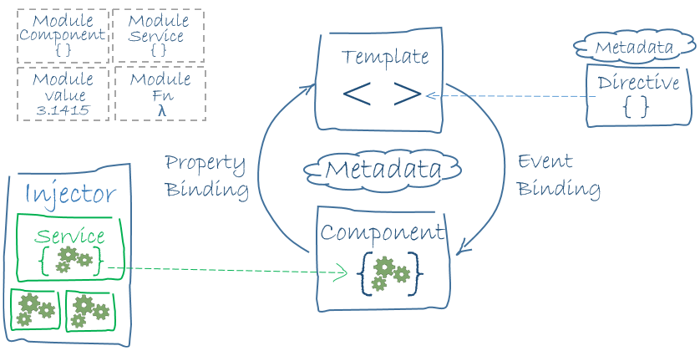
\includegraphics [height=8cm, width=15cm] {images/angular-component-structure}
\pagebreak

\subsubsection{Example of an Angular Component:}
Here is an Example of the essential files of an Angular component:\\\\
\textbf{component.html:}
\begin{Verbatim}[frame=single]
 <h1>{{text}}</h1>
\end{Verbatim}
\textbf{component.ts:}
\begin{Verbatim}[frame=single]
 @NgComponent({
   selector:'my-text',
   templateUrl: './my-text.component.html',
   styleUrls: ['./my-text.component.css']
 })
    
   export class myText{
   myText:string
 }
\end{Verbatim}
The @NgComponent decorator tells the compiler that the following class belongs to a component. The decorator takes an object as a parameter which provides essential metadata for the component. The selector determines the name with which the component can be used in an HTML file, the templateUrl contains the path of the component.html file and the styleUrls is an array in which the paths to all the CSS files belonging to the component. The following class containes the variable that is used to pass text to the h1 element in the component.html file.
%xxxxxxxxxxxxxxxxxxxxxxxxxxxxxxxxxxxxxxxxxxxxxxxxxxxxxx
\section{React}
React is an open source Library for building user interfaces released by Facebook in 2013 to make the development of their social platform easier. React is not a fully fledged framework, because it does not dictate any design system or even provide an eco-system or built in features. Much of the functionality of a React application must be drawn from third party libraries.
\subsection{Components in React}
In Angular technologies are artificially separated by having a file for HTML and TypeScript for a component. React however separates concerns, meaning that what belongs together is stored together resulting in components that consist of a single file that contains the TypeScript code as well as the CSS styling and the HTML code of a component. To achieve this, React uses JSX or TSX, depending on whether the project is built in JavaScript or TypeScript. In this thesis TSX will be used. Furthermore, in React, components can be implemented as either class components or functional components. Before React 16.8 a class component would be required for state management. Since update 16.8 however the difference between functional and class components is only syntactical and it is recommended to use functional components going forward. In contrary to Angular, React components are not updated, but created as new instances.\\[0.5cm]
In the following examples the syntactical difference between class and functional components will be demonstrated. In both cases the HTML will look like this:
\begin{Verbatim}[frame=single]
 <MyText input="Hello, World!"/>
\end{Verbatim}
\textbf{Example of a functional Component:}
\begin{Verbatim}[frame=single]
 function MyText(props:myTextProps){
   return (<h1>{myTextProps.input}</h1>);
 }
\end{Verbatim}
\textbf{Example of a Class Component:}
\begin{Verbatim}[frame=single]
 class MyText extends React.Component{
   render(){
     return(<h1>{this.props.input}</h1>)
   }			
 }
\end{Verbatim}
Note that there is no props object explicitely passed to the class. This is because the props object is auto generated from the HTML code.
\subsection{Basic Concepts}
\subsubsection{TSX}
Without TSX every HTML element has to be created by calling the React.createElement function or as an object. TSX is an abstraction of TypeScript that enhances the syntax and enables the TypeScript compiler to parse HTML code in a TypeScript file into calls of the React.createElement function. Thus Typescript and HTML code can be stored in the same file. In TSX, a React component has a method called "render" that contains the HTML code to be rendered.\\\\
\textbf{Example for React.createElement call:}
\begin{Verbatim}[frame=single]
 const element = React.createElement(
   h1,
   {className: 'greeting'},
   'Hello World!'
 );
\end{Verbatim}
\pagebreak
\textbf{Example for element as object:}
\begin{Verbatim}[frame=single]
 const element = {
   type: 'h1',
   props: {
     classname: 'greeting',
     children: 'Hello, World!'
   }
 };
\end{Verbatim}
\textbf{Example of render function in TSX:}
\begin{Verbatim}[frame=single]
 render() {
   return (
     <h1>Hello, World!</h1>
   )    
 }
\end{Verbatim}
\subsubsection{States}
In React, a component maintains its own data using a state. A state is different to props in that the data is private and managed only by the component itself.
By giving the component control over its own data it can rerender itself and does no longer need to be reinstantiated every time the data changes. Since React 16.8 the use of a state no longer requires a class component with a constructor, essentially making class components obsolete. An example will be given in the hook section\\

The count variable is used as the state here. The Array defines the variable and a function that can be called to change the value of count. The useState hook (more on hooks below)is used to add the state to the component and initialize it. When the button is clicked, it will use the setCount function to update the state, which will in turn cause the component to rerender with the new state.
\pagebreak
\subsubsection{Hooks}
Hooks were introduced in React 16.8 and are JavaScript functions that are used to handle state data in components. They  extract the stateful logic from components and make it reusable. The basic Hooks are:
\begin{itemize}
\item \textbf{useState():} is used to update a state, triggering a rerendering of the component.
This example demonstrates the use of useState:
\begin{Verbatim}[frame=single]
 function Counter(){
   const [count, setCount] = useState(0);
   return (
     <div>
       <p>{count}</p>		            
       <button onClick={() => setCount(count + 1)}>+</button>
     </div>
   );
 }
\end{Verbatim}

\item \textbf{useEffect():} useEffect always runs when any stateful data changes. This behavior can be controlled more accurately by providing the hook with an array of dependencies in which the exact states that the hook should watch for changes are specified. If useEffect is called with no dependency array, it will run when the component is mounted into the UI and when the state changes. An empty dependency array will cause the hook to only run once when the component is initialized since there are no states being watched. If the array has dependencies only those states will be watched for changes and the hook will not necessarily run upon mounting the component.\\This example shows the same component as before with a second state variable and a useEffect hook:
\begin{Verbatim}[frame=single]
 function Counter(){
   const [count, setCount] = useState<number>(0);
   const [loaded, setLoaded] = useState<boolean>(false);
   
   useEffect(
     ()=>{
       fetch('foo').then(()=>setLoaded(true))
     },
     [count] // dependency array
   )
   return (
     <div>
       <p>{count}</p>		            
       <button onClick={() => setCount(count + 1)}>+</button>
     </div>
   );
 }
\end{Verbatim}
\pagebreak
\item \textbf{useContext():} The useContext hook allows for stateful data to be shared or scoped using React's Context API. This means that a variable can be used by multiple disconnected components and if there is a change all the components that use the variable are updated. To do this, a variable or set of variables must be declared in the top most parent component (i.e. the App component if the data is to be used everywhere). Any child component inside the resulting component tree will inherit this variable without the need to pass it via property. By calling the useContext hook the data can be accessed and should it change, the changes will be applied to all child components automatically. The following example demonstrates the use of useContext.\\[0.5cm]
In App.js:
\begin{Verbatim}[frame=single]
 const fruits = { //data for context
   monday: 'Apple',
   tuesday: 'strawberry'
 }
 //creating context
 const FruitContext fruits = createContext(fruits)

 function App (props) {
   return (
     //the context is shared to all components inside the
     FruitContext tag.
     <FruitContext.Provider value = {fruit.monday}>
       <todays-fruit/>
     </FruitContext.Provider>
   );  
 }
\end{Verbatim}
In todays-fruit component
\begin{Verbatim}[frame=single]
 function todays-fruit () {
   const todaysFruit = useContext(FruitContext)
   return <p>{todaysFruit}</p>
 }
\end{Verbatim}
\end{itemize}

\subsubsection{Other Concepts}
Services, decorators and metadata have already been covered in the Angular section and are not much different in React.
\chapter{Vue}
Vue is a very simple frontend web framework created by ex-Google employee Evan You in 2014 with the goal of building a custom tool around the best parts of Angular. Vue is designed for creating smaller projects and can be used to create entire applications or just single widgets to be used in other websites.
\subsection{Copmonents in Vue}
Vue works with single file copmonents, meaning that all the code of a component is stored in a single file. While styling can be done externally in both Angular and React, this is not the case in Vue.\\[0.5cm]
The structure of a Vue component is much simpler than that of a React component as it is divided into three html tags: template, script and style. The template tag contains the HTML code of the component while the script tag contains any JavaScript or TypeScript and the style tag contains the CSS styling.\\[0.5cm]
\textbf{Example of a simple Vue component}
\begin{Verbatim}[frame=single]
 <template>
   <p>Hello, World!<p>
 </template>
 
 <script lang="ts">
   import {defineComponent} from 'vue';
   
   export default defineComponent({
     name: 'hello-world',
     components:{},
     methods:{
       hello(){console.log('Hello, World!');}
     }
   });
 </script>
 
 <style>
   p {
     text-align: center;
     color: green;
   }
 <style/>
\end{Verbatim}
\subsubsection{Registration}
For Vue to locate a component's implementation when it is encountered in a template it needs to be registered.
Components can be registered either globally or locally.









\chapter{Working with \latex}
\label{cha:WorkingWithLatex}


\chapter{Figures, Tables, Source Code}
\label{cha:Figures}

\chapter[Mathematical Elements]{Mathematical Elements, Equations and Algorithms}
\label{cha:Mathematics}


\chapter[Using Literature]{Using Literature and other Resources}
\label{cha:Literature}


\cite{Drake1948}	% a reference for testing


\chapter{Printing the Manuscript}
\label{cha:Printing}


\chapter{Closing Remarks}
\label{cha:Closing}

%%%-----------------------------------------------------------------------------
\appendix                                                             % Appendix 
%%%-----------------------------------------------------------------------------

\chapter{Technical Details}
\label{app:TechnicalDetails}



 % Technical supplements
\chapter{Supplementary Materials}
\label{app:materials}


List of supplementary data submitted to the degree-granting institution for archival storage
(in ZIP format).

% Use this as an example only, adapt the structure to your requirements!

\section{PDF Files}
\begin{FileList}{/}
\fitem{thesis.pdf} Master/Bachelor thesis (complete document)
\end{FileList}

\section{Media Files}
\begin{FileList}{/media}
\fitem{*.ai, *.pdf} Adobe Illustrator files
\fitem{*.jpg, *.png} raster images
\fitem{*.mp3} audio files
\fitem{*.mp4} video files
\end{FileList}


\section{Online Sources (PDF Captures)}
\begin{FileList}{/online-sources}
\fitem{Reliquienschrein-Wikipedia.pdf} \citenobr{WikiReliquienschrein2022}
\end{FileList}




 % Contents of the CD-ROM/DVD
\chapter{Questionnaire}
\label{app:Questionnaire}





 % Chronological list of changes
\chapter{\latex Source Code}
\label{app:SourceCode}

 % Source text of this document

%%%-----------------------------------------------------------------------------
\backmatter                           % Back part (bibliography, glossary, etc.)
%%%-----------------------------------------------------------------------------

\MakeBibliography % References

%%%-----------------------------------------------------------------------------
% Special page for checking print size
%%%-----------------------------------------------------------------------------

\chapter*{Check Final Print Size}

\begin{center}
{\Large --- Check final print size! ---}

\bigskip

\calibrationbox{100}{50} % width/height of box in mm

\bigskip

{\Large --- Remove this page after printing! ---}

\end{center}



%%%-----------------------------------------------------------------------------
\end{document}
%%%-----------------------------------------------------------------------------
